\documentclass[aspectratio=169,usepdftitle=true]{beamer}

\usepackage[T1]{fontenc}
\usepackage[utf8]{inputenc}
\usepackage{microtype}
\usepackage[english]{babel}
\usepackage{lipsum}
\usepackage{multirow}
\usepackage{amsmath}
\usetheme{dividing-lines}
\usepackage{amsfonts}
\usepackage{bbold}
\usepackage{booktabs}
%\usepackage[scale=2]{ccicons}
\usepackage{graphicx}
\usepackage{pgfplots}
%\usepgfplotslibrary{dateplot}

\title{A new statistical model to assess the burden of misreported epidemiological data}
%\subtitle{This is madness}
\institute{Reuni\'on anual SEE 2022}
\license{\ccbysa}

\date{August 31st 2022}

\author{David Mori\~na, Amanda Fern\'andez-Fontelo, Alejandra Caba\~na, Argimiro Arratia and Pere Puig}
\email{dmorina@ub.edu}

\outro{Thank you!}
\titleimage{\tikz\node[opacity=.45]{
\includegraphics[width=4cm,height=\height,keepaspectratio]{BUlogo_cmyk-eps-converted-to.pdf}};}

% just an example command
\newcommand\twosplit[3][t]{%
\begin{columns}[#1]
\begin{column}{0.475\linewidth}#2\end{column}\hfill
\begin{column}{0.475\linewidth}#3\end{column}
\end{columns}}

\usepackage[backend=bibtex8,style=alphabetic]{biblatex}
%\addbibresource{example.bib}
\begin{document}

\section{Introduction}

\begin{frame}{Introduction}
\begin{itemize}
 \item The Covid-19 pandemic that is hitting the world since late 2019 has made evident that having quality data is essential in the decision making chain, especially in epidemiology but also in many other fields. There is an enormous global concern around this disease, leading the World Health Organization (WHO) to declare public health emergency
 \item As a large proportion of the cases run asymptomatically and mild symptoms could have been easily confused with those of similar diseases at the beginning of the pandemic, its reasonable to expect that Covid-19 incidence has been notably underreported
\end{itemize}
\end{frame}

\subsection{Previously proposed models}
\begin{frame}[c]{Previously proposed models (count data)}
    \begin{block}{Independent under-reporting states}
        \begin{center}
           
\includegraphics[height=4.7cm,width=7.5cm]{SiM1.png}
        \end{center}
    \end{block}
\end{frame}

\begin{frame}[c]{Previously proposed models (count data)}
    \begin{block}{Serially dependent under-reporting states}
        \begin{center}
           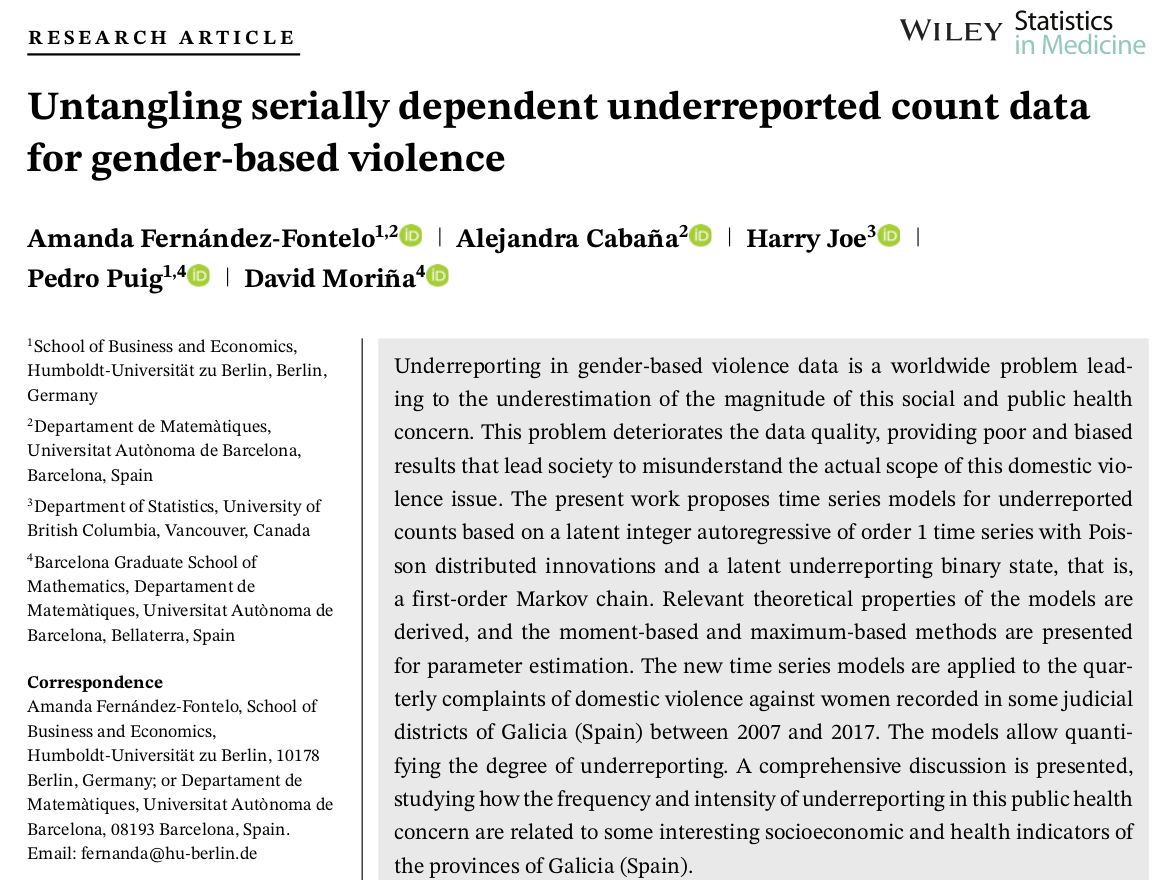
\includegraphics[height=4.7cm,width=7.5cm]{SiM2.png}
        \end{center}
    \end{block}
\end{frame}

\begin{frame}[c]{Previously proposed models (count data)}
    \begin{block}{Non-stationary processes}
        \begin{center}
           
\includegraphics[height=4.7cm,width=7.5cm]{Plos.png}
        \end{center}
    \end{block}
\end{frame}

\begin{frame}[c]{Previously proposed models (continuous data)}
    \begin{block}{Non-correlated longitudinal data}
        \begin{center}
           
\includegraphics[height=4.7cm,width=7.5cm]{MRM.png}
        \end{center}
    \end{block}
\end{frame}

\begin{frame}[c]{Previously proposed models (continuous data)}
    \begin{block}{Classical time series}
        \begin{center}
           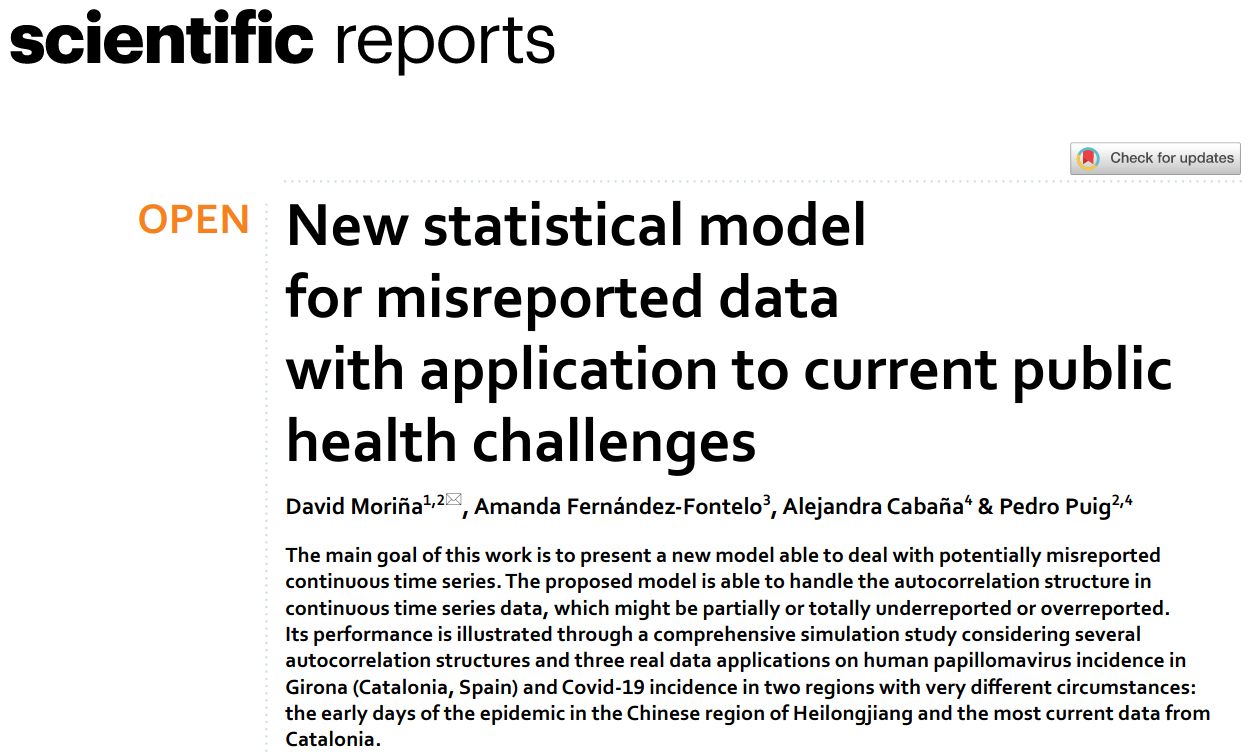
\includegraphics[height=4cm,width=8cm]{SR.png}
        \end{center}
    \end{block}
\end{frame}

\section{Methods}

\subsection{Proposed model}
\begin{frame}{Model}
Consider an unobservable process $X_t$ following an AutoRegressive ($AR(1)$) model with ARCH(1) errors structure, defined by
\begin{equation}\label{eq:ARCH}
X_t = \phi_0 + \phi_1 \cdot X_{t-1} + Z_t,
\end{equation}
where $Z^2_t=\alpha_0+\alpha_1 \cdot Z^2_{t-1} + \epsilon_t,$ being $\epsilon_t \sim N(\mu_{\epsilon}(t), \sigma^2)$.

In our setting, this process $X_t$ cannot be directly observed, and all we can see is a part of it, expressed as

\begin{equation}\label{eq:model}
    Y_t=\left\{
                \begin{array}{ll}
                  X_t \text{ with probability } 1-\omega \\
                  q \cdot X_t \text{ with probability } \omega
                \end{array}
              \right.
\end{equation}
\end{frame}

\begin{frame}{Model}
The expectation of the innovations $\epsilon_t$ is linked to a simplified version of the well-known compartimental Susceptible-Infected-Recovered (SIR) model. At any time $t \in \mathbb{R}$ there are three kinds of individuals: Healthy individuals susceptible to be infected ($S(t)$), infected individuals who are transmitting the disease at a certain speed ($I(t)$) and individuals who have suffered the disease, recovered and cannot be infected again ($R(t)$). The number of affected individuals at time $t$, $A(t) = I(t) + R(t)$ can be approximated by

\begin{equation}\label{eq:SIR}
    A(t) = \frac{M^{*}(\beta_0, \beta_1, t) A_0 e^{kt}}{M^{*}(\beta_0, \beta_1, t)+A_0(e^{kt}-1)},
\end{equation}
\end{frame}

\begin{frame}{BSL}
\begin{itemize}
 \item Synthetic likelihood is a recent and very powerful alternative for parameter estimation in a simulation based schema when the likelihood is intractable but the generation of new observations given the values of the parameters is feasible
 \item Introduced by Simon Wood in 2010, Bayesian framework by Leah F. Price \textit{et al.} in 2018
 \item The method takes a vector summary statistic informative about the parameters and assumes it is multivariate normal, estimating the unknown mean and covariance matrix by simulation to obtain an approximate likelihood function of the multivariate normal
\end{itemize}
\end{frame}

\section{Results}
\subsection{Covid-19 incidence in Spain}
\begin{frame}{Covid-19 in Spain}
The betacoronavirus SARS-CoV-2 has been identified as the causative agent of an unprecedented world-wide outbreak of pneumonia starting in December 2019 in the city of Wuhan (China), named as Covid-19. Considering that many cases run without developing symptoms or just with very mild symptoms, it is reasonable to assume that the incidence of this disease has been underregistered. This work focuses on the weekly Covid-19 incidence registered in Spain in the period (2020/02/23-2022/04/03) 
\end{frame}

\begin{frame}[fragile]{Covid-19 in Spain}
\centering
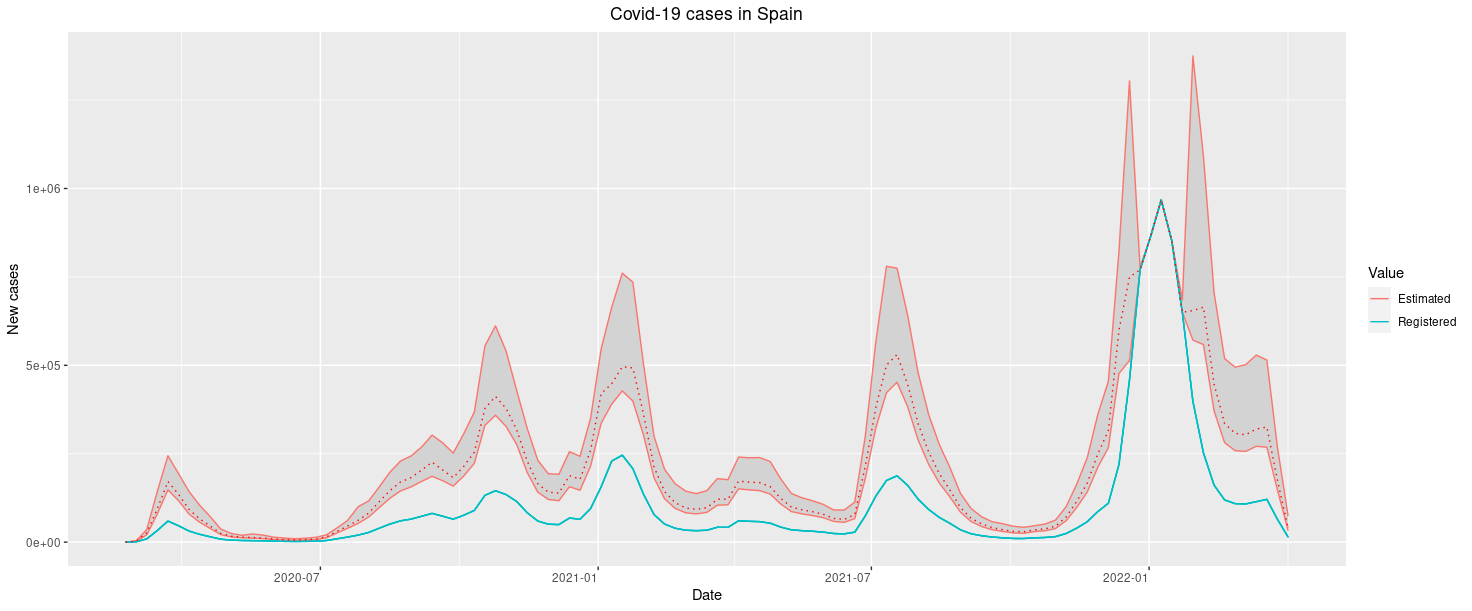
\includegraphics[scale=0.3]{global_Spain.png}
\end{frame}

\begin{frame}{Covid-19 in Spain}
 \vspace{-1cm}
  \begin{columns}
      \hspace{-1cm}
    \begin{column}{0.6\textwidth}
        \begin{table}\tiny
\resizebox{5.5cm}{!}{\begin{tabular}{ccc}
\toprule
CCAA & Parameter & Estimate (95\% CI)\\
\midrule
\multirow{2}{*}{Andaluc\'ia}  & $\hat{\omega}$  & 0.97 (0.95 - 0.99) \\
                              & $\hat{q}$       & 0.44 (0.41 - 0.48) \\
\midrule
\multirow{2}{*}{Arag\'on}    & $\hat{\omega}$  & 0.98 (0.97 - 0.99) \\
                             & $\hat{q}$       & 0.28 (0.27 - 0.32) \\
\midrule
\multirow{2}{*}{Asturies}    & $\hat{\omega}$  & 0.97 (0.90 - 0.99) \\
                             & $\hat{q}$       & 0.40 (0.37 - 0.53) \\
\midrule
\multirow{2}{*}{Cantabria}    & $\hat{\omega}$  & 0.97 (0.95 - 0.99) \\
                              & $\hat{q}$       & 0.30 (0.28 - 0.35) \\
\midrule
\multirow{2}{*}{Castilla y Le\'on}    & $\hat{\omega}$  & 0.98 (0.95 - 0.99) \\
                                      & $\hat{q}$       & 0.36 (0.32 - 0.41) \\
\midrule
\multirow{2}{*}{Castilla - La Mancha}    & $\hat{\omega}$  & 0.98 (0.96 - 0.99) \\
                                         & $\hat{q}$       & 0.33 (0.31 - 0.36) \\
\midrule
\multirow{2}{*}{Canarias}    & $\hat{\omega}$  & 0.98 (0.96 - 0.99) \\
                             & $\hat{q}$       & 0.35 (0.32 - 0.38) \\
\midrule
\multirow{2}{*}{Catalunya}    & $\hat{\omega}$  & 0.98 (0.96 - 0.99) \\
                              & $\hat{q}$       & 0.30 (0.27 - 0.34) \\
\midrule
\multirow{2}{*}{Ceuta}    & $\hat{\omega}$  & 0.98 (0.95 - 0.99) \\
                          & $\hat{q}$       & 0.28 (0.25 - 0.31) \\
\bottomrule
\end{tabular}}
\end{table}
    \end{column}
    \begin{column}{0.6\textwidth}
    \hspace{-1cm}
          \begin{table}\tiny
\resizebox{5.5cm}{!}{\begin{tabular}{ccc}
\toprule
CCAA & Parameter & Estimate (95\% CI)\\
\midrule
\multirow{2}{*}{Extremadura}    & $\hat{\omega}$  & 0.98 (0.95 - 1.00) \\
                                & $\hat{q}$       & 0.40 (0.36 - 0.44) \\
\midrule
\multirow{2}{*}{Galiza}     & $\hat{\omega}$  & 0.84 (0.33 - 0.98) \\
                            & $\hat{q}$       & 0.41 (0.35 - 0.56) \\
\midrule
\multirow{2}{*}{Illes Balears}    & $\hat{\omega}$  & 0.98 (0.96 - 0.99) \\
                                  & $\hat{q}$       & 0.36 (0.33 - 0.39) \\
\midrule
\multirow{2}{*}{Regi\'on de Murcia}    & $\hat{\omega}$  & 0.93 (0.45 - 0.98) \\
                                       & $\hat{q}$       & 0.46 (0.34 - 0.80) \\
\midrule
\multirow{2}{*}{Madrid}      & $\hat{\omega}$  & 0.98 (0.96 - 0.99) \\
                             & $\hat{q}$       & 0.37 (0.34 - 0.40) \\
\midrule
\multirow{2}{*}{Nafarroa}    & $\hat{\omega}$  & 0.99 (0.97 - 1.00) \\
                             & $\hat{q}$       & 0.30 (0.26 - 0.32)\\
\midrule
\multirow{2}{*}{Euskadi}    & $\hat{\omega}$  & 0.99 (0.97 - 0.99) \\
                            & $\hat{q}$       & 0.27 (0.25 - 0.31) \\
\midrule
\multirow{2}{*}{La Rioja}    & $\hat{\omega}$  & 0.98 (0.96 - 0.99) \\
                             & $\hat{q}$       & 0.31 (0.28 - 0.35) \\
\midrule
\multirow{2}{*}{Melilla}    & $\hat{\omega}$  & 0.97 (0.95 - 0.99) \\
                            & $\hat{q}$       & 0.34 (0.31 - 0.37) \\
\midrule
\multirow{2}{*}{Pa\'is Valenci\`a}    & $\hat{\omega}$  & 0.95 (0.40 - 0.98) \\
                                      & $\hat{q}$       & 0.46 (0.40 - 0.67) \\
\bottomrule
\end{tabular}}
\end{table}
\end{column}
\end{columns}
\end{frame}

\begin{frame}{Covid-19 in Spain}
\begin{itemize}
\item In the considered period, the official sources reported 11,612,568 Covid-19 cases in Spain, while the model estimates a total of 23,674,309 cases (only 51\% of actual cases were reported) \item While the frequency of underreporting is extremely high for all regions (minimum value of $\hat{\omega}=0.84$ in Galiza), the intensity of this underreporting is not uniform across the considered regions. It can be seen that Arag\'on and Ceuta are the regions with highest underreporting intensity ($\hat{q}=0.28$) while Pa\'is Valenci\`a and Regi\'on de Murcia are the ones where the estimated values are closest to the number of reported cases ($\hat{q}=0.46$)
\end{itemize}
\end{frame}

\begin{frame}[fragile]{Covid-19 in Spain}
\centering
\hspace{-1.6cm}
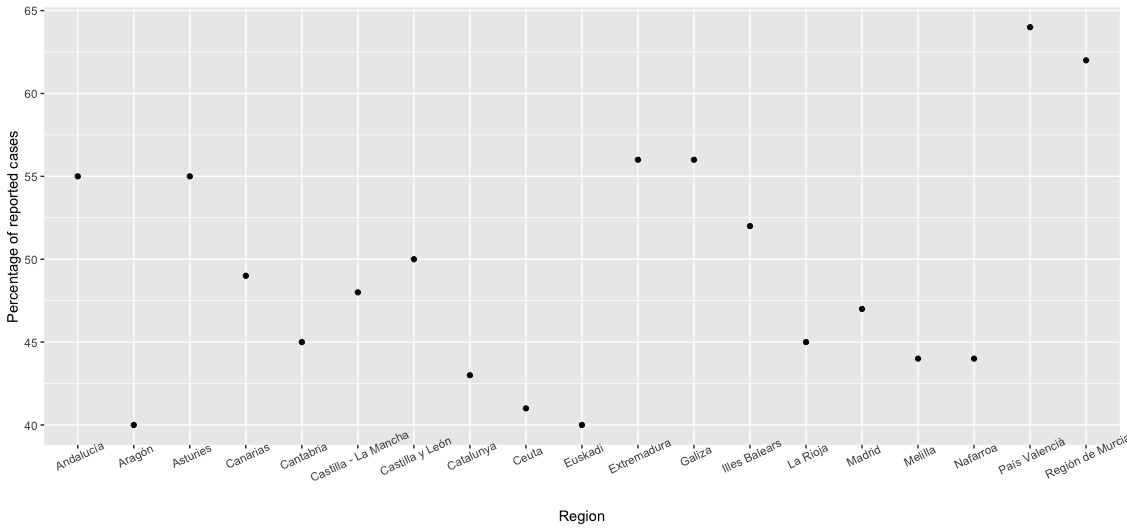
\includegraphics[scale=0.3]{perc_reported.png}
\end{frame}

\begin{frame}{Impact of covariates}
 \vspace{-1cm}
  \begin{columns}
      \hspace{-1cm}
    \begin{column}{0.6\textwidth}
        \begin{table}\tiny
\resizebox{5.5cm}{!}{\begin{tabular}{ccc}
\toprule
CCAA & Covariate & Estimate (95\% CI)\\
\midrule
Andaluc\'ia  & $\hat{Vacc}$  & -1.71 (-2.66, -0.68) \\
\midrule
Arag\'on    & $\hat{Vacc}$  & -1.06 (-1.36, -0.69) \\
\midrule
Asturies    & $\hat{Vacc}$  & -0.90 (-1.77, -0.63) \\
\midrule
Cantabria    & $\hat{Vacc}$  & -0.53 (-1.29, -0.25) \\
\midrule
Castilla y Le\'on    & $\hat{Vacc}$  & -1.22 (-1.88, -0.60) \\
\midrule
Castilla - La Mancha    & $\hat{Vacc}$  & -0.80 (-1.11, -0.40) \\
\midrule
Canarias    & $\hat{Vacc}$  & -1.34 (-1.78, -1.06) \\
\midrule
Catalunya    & $\hat{Vacc}$  & -1.51 (-1.97, -0.94) \\
\midrule
Ceuta    & $\hat{Vacc}$  & -1.38 (-1.93, -0.84) \\
\bottomrule
\end{tabular}}
\end{table}
    \end{column}
    \begin{column}{0.6\textwidth}
    \hspace{-1cm}
          \begin{table}\tiny
\resizebox{5.5cm}{!}{\begin{tabular}{ccc}
\toprule
CCAA & Parameter & Estimate (95\% CI)\\
\midrule
Extremadura    & $\hat{Vacc}$  & -0.72 (-1.30, -0.37) \\
\midrule
Galiza     & $\hat{Vacc}$  & -2.03 (-3.07, -1.34) \\
\midrule
Illes Balears    & $\hat{Vacc}$  & -0.72 (-1.16, -0.34) \\
\midrule
Regi\'on de Murcia    & $\hat{Vacc}$  & -1.97 (-3.07, -0.59) \\
\midrule
Madrid      & $\hat{Vacc}$  & -0.35 (-0.77, -0.07) \\
\midrule
Nafarroa   & $\hat{Vacc}$  & -2.05 (-3.20, -1.33) \\
\midrule
Euskadi    & $\hat{Vacc}$  & -0.10 (-0.24, 0.00) \\
\midrule
La Rioja    & $\hat{Vacc}$  & -0.43 (-0.71, -0.22) \\
\midrule
Melilla   & $\hat{Vacc}$  & -1.59 (-2.05, -0.93) \\
\midrule
Pa\'is Valenci\`a    & $\hat{Vacc}$  & -1.70 (-2.64, -0.52) \\
\bottomrule
\end{tabular}}
\end{table}
\end{column}
\end{columns}
\end{frame}

\section{Further work}
\begin{frame}{Next steps}
\begin{itemize}
 \item Model diagnostics
 \item Simulation study
 \item Underlying process model selection procedure
 \item Model adjustments for more realistic assumptions
\end{itemize}
\end{frame}

\end{document}